\documentclass[conference,10pt]{IEEEtran}
\IEEEoverridecommandlockouts

\usepackage[utf8]{inputenc}
\usepackage[T1]{fontenc}
\usepackage[brazil]{babel}
\usepackage{cite}
\usepackage{amsmath,amssymb,amsfonts}
\usepackage{graphicx}
\usepackage{textcomp}
\usepackage{xcolor}
\usepackage{booktabs}
\usepackage{multirow}
\usepackage{array}
\usepackage{url}
\usepackage[hidelinks]{hyperref}

\graphicspath{{figures/}}

\begin{document}

\title{Modelagem e Avaliação de Desempenho de Servidores Web com Controle de Admissão Utilizando Redes de Petri Estocásticas}

\author{\IEEEauthorblockN{Leonardo Virgulino Rodrigues Carvalho}
\IEEEauthorblockA{\textit{Universidade Federal do Piauí (UFPI)}\\
Picos, PI, Brasil}
}

\maketitle

\begin{abstract}
Aplicações Web lidam com variações constantes no volume de acessos e precisam de dimensionamento adequado para evitar lentidão e rejeição de conexões. Realizar testes de carga diretamente na infraestrutura real tem custo alto e dificulta a comparação de várias configurações de hardware. O uso de Redes de Petri Estocásticas (Stochastic Petri Nets, SPN) permite simular e prever o comportamento de sistemas concorrentes antes da sua implementação física. Este trabalho apresenta um modelo SPN construído na ferramenta Jupiter Analytics para avaliar o desempenho de um conjunto de Servidores Web com controle de admissão e fila limitada. Foram calculadas seis métricas em regime estacionário: vazão (TP), tempo médio de resposta (MRT), tempo médio de fila (MQT), tempo médio de processamento (MPT), utilização dos servidores (U) e probabilidade de descarte (DP). A avaliação contou com quatro baterias de experimentos (E1 a E4), variando a taxa de chegada de requisições, a quantidade de núcleos de processamento e o tamanho máximo da fila. Os resultados mostram que a quantidade de núcleos de processamento é o principal gargalo do sistema e que aumentar apenas o limite da fila eleva o tempo de resposta em até 121,8\% sem ganho expressivo na vazão. A configuração com 12 núcleos e fila de 20 posições atendeu 98,86\% da demanda sob tráfego elevado, reduzindo o tempo médio de resposta em 42,4\% e mantendo o descarte em 1,14\%.
\end{abstract}

\begin{IEEEkeywords}
Redes de Petri Estocásticas, Servidor Web, Avaliação de Desempenho, Jupiter Analytics, Dimensionamento de Capacidade.
\end{IEEEkeywords}

\section{Introdução}
Serviços de comércio eletrônico, portais acadêmicos, sistemas bancários e aplicações em nuvem dependem diretamente do desempenho de servidores Web \cite{menasce2002}. Em horários de pico, centenas ou milhares de usuários enviam requisições HTTP/HTTPS ao mesmo tempo e esperam respostas rápidas, geralmente na faixa de dezenas de milissegundos \cite{cao2003}. Quando a taxa de chegada de requisições ultrapassa a velocidade de atendimento dos servidores, as solicitações acumulam na fila do balanceador de carga. Esse acúmulo aumenta o tempo de espera do cliente e gera descarte de pacotes (erro HTTP 503) quando o espaço de fila acaba.

Definir a quantidade certa de recursos em um servidor Web envolve equilibrar o custo da infraestrutura e a qualidade do atendimento \cite{santos2021}. Poucos servidores causam sobrecarga rápida de CPU, filas longas e perda de requisições. Por outro lado, alocar máquinas em excesso deixa os processadores ociosos na maior parte do tempo e aumenta o gasto com servidores ou instâncias em nuvem \cite{macedo2022}. Testar todas essas combinações em ambientes reais exige montar a infraestrutura antes e gerar tráfego artificial em larga escala, o que nem sempre é viável durante a fase de projeto.

As ferramentas de modelagem analítica e simulação permitem estudar o comportamento de sistemas distribuídos com baixo custo e boa precisão \cite{bolch2006}. As Redes de Petri Estocásticas (SPN) são bastante usadas para essa finalidade porque representam de forma visual e matemática o paralelismo, a sincronização, a disputa por recursos e os limites de fila presentes em servidores reais \cite{marsan1995, oliveira2017}. Com o modelo construído em ferramentas como o Jupiter Analytics \cite{jupiter2024}, o projetista consegue alterar parâmetros de chegada, fila e processamento para identificar gargalos antes de implantar o sistema.

Vários trabalhos na literatura usam modelos analíticos para estudar servidores e redes de comunicação. Cao et al. \cite{cao2003} usaram um modelo de fila $M/G/1/K*PS$ para estimar o tempo de resposta e a taxa de rejeição em servidores Web. Menascé e Almeida \cite{menasce2002} apresentaram modelos baseados em redes de filas para o planejamento de capacidade de serviços na Internet. Oliveira et al. \cite{oliveira2017} desenvolveram técnicas de modelagem com Redes de Petri Estocásticas para avaliação de sistemas computacionais. Santos et al. \cite{santos2021} usaram SPN para medir o desempenho do processamento de dados entre camadas Edge e Cloud. Macêdo et al. \cite{macedo2022} também aplicaram SPN para avaliar tempo médio de resposta, utilização e probabilidade de descarte na comunicação de redes veiculares, analisando o impacto de variar o número de máquinas e núcleos em cada camada.

Seguindo essa linha de modelagem de filas e recursos \cite{macedo2022, oliveira2017}, este trabalho propõe e avalia um modelo SPN no Jupiter Analytics voltado para um sistema de \textbf{Servidor Web com controle de admissão e múltiplos servidores}. Os objetivos e contribuições do trabalho são:
\begin{itemize}
    \item Construir um modelo SPN parametrizado que representa a chegada de requisições HTTP, o controle de admissão em fila finita, a disputa por núcleos de processamento e o descarte por falta de vagas;
    \item Calcular seis métricas de desempenho (TP, MRT, MQT, MPT, U e DP) em quatro grupos de experimentos (E1 a E4);
    \item Identificar o principal gargalo da arquitetura e apontar a configuração de servidores e fila com melhor relação entre uso de recursos e tempo de resposta.
\end{itemize}

O artigo está dividido da seguinte maneira: a Seção II apresenta a arquitetura do sistema Web e a pergunta de pesquisa. A Seção III explica o modelo SPN, seus componentes e as fórmulas das métricas. A Seção IV mostra a configuração dos experimentos E1 a E4 e discute os gráficos e resultados obtidos. A Seção V traz as conclusões do trabalho e os links para o repositório e vídeo de apresentação.

\section{Arquitetura do Sistema}

\subsection{Visão Geral e Funcionamento}
A Figura~\ref{fig:arquitetura} mostra a arquitetura considerada para o sistema de Servidor Web. O fluxo é dividido em três partes: os clientes na Internet, a camada de admissão com fila limitada e o grupo (pool) de servidores Web que processam as requisições.

\begin{figure}[htbp]
    \centering
    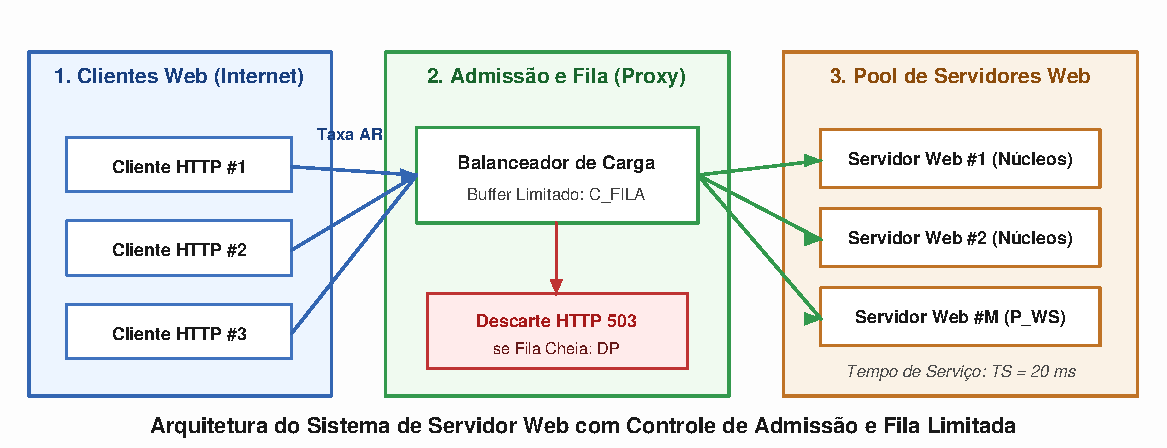
\includegraphics[width=\columnwidth]{fig_arquitetura_web.pdf}
    \caption{Arquitetura do sistema de Servidor Web dividida em Clientes Web, Camada de Admissão com fila limitada e Pool de Servidores Web.}
    \label{fig:arquitetura}
\end{figure}

\begin{enumerate}
    \item \textbf{Clientes Web}: Representam os usuários que enviam requisições HTTP/HTTPS pela Internet. As solicitações chegam com uma taxa média $AR$ (medida em requisições por milissegundo, req/ms). O tempo médio entre duas chegadas seguidas é dado por $AD = 1/AR$~ms.
    \item \textbf{Camada de Admissão e Fila (Proxy / Balanceador)}: Funciona como porta de entrada do serviço (como um servidor NGINX ou HAProxy). Quando uma requisição chega, o balanceador verifica se existe vaga na fila de espera, que suporta no máximo $C\_FILA$ requisições. Se houver vaga, a requisição entra na fila. Se todas as $C\_FILA$ posições estiverem ocupadas, a requisição é descartada na entrada (erro HTTP 503) para evitar o travamento dos servidores.
    \item \textbf{Pool de Servidores Web}: Formado pelas máquinas que executam a aplicação Web. A capacidade total de atendimento paralelo é definida por $P\_WS$ núcleos ($\text{Capacidade} = \text{Máquinas} \times \text{Núcleos}$). As requisições da fila são atendidas por ordem de chegada (política FCFS, \textit{First-Come, First-Served}), sem preempção. Cada núcleo gasta em média $TS$~ms para processar uma requisição e liberar o recurso.
\end{enumerate}

\subsection{Restrições e Hipóteses Consideradas}
Para construir e avaliar o modelo SPN, foram adotadas as seguintes suposições:
\begin{itemize}
    \item Todos os núcleos dos servidores Web têm a mesma configuração e velocidade média de processamento ($\mu = 1/TS$~req/ms);
    \item O intervalo entre chegadas de requisições ($AD = 1/AR$) e o tempo de processamento em cada servidor ($TS = 20$~ms) seguem distribuição exponencial;
    \item A fila de espera atende na ordem FCFS não-preemptiva e descarta novas requisições apenas quando atinge o limite $C\_FILA$;
    \item O atraso da rede externa dos clientes não foi incluído para focar a análise apenas na fila e nos servidores Web.
\end{itemize}

\subsection{Pergunta de Pesquisa}
A análise conduzida neste trabalho busca responder à seguinte pergunta:
\begin{quote}
\textit{``De que forma a taxa de chegada de requisições ($AR$), a quantidade de núcleos de processamento ($P\_WS$) e o tamanho máximo da fila ($C\_FILA$) afetam a vazão, o tempo de resposta e o descarte em um Servidor Web, e qual configuração oferece o melhor equilíbrio entre recursos alocados e desempenho?''}
\end{quote}

\section{Modelagem do Sistema}

\subsection{Modelo SPN Proposto}
A Figura~\ref{fig:spn} mostra o modelo SPN criado na ferramenta Jupiter Analytics para representar a arquitetura da Figura~\ref{fig:arquitetura}. O fluxo das fichas (\textit{tokens}) segue da esquerda para a direita.

\begin{figure}[htbp]
    \centering
    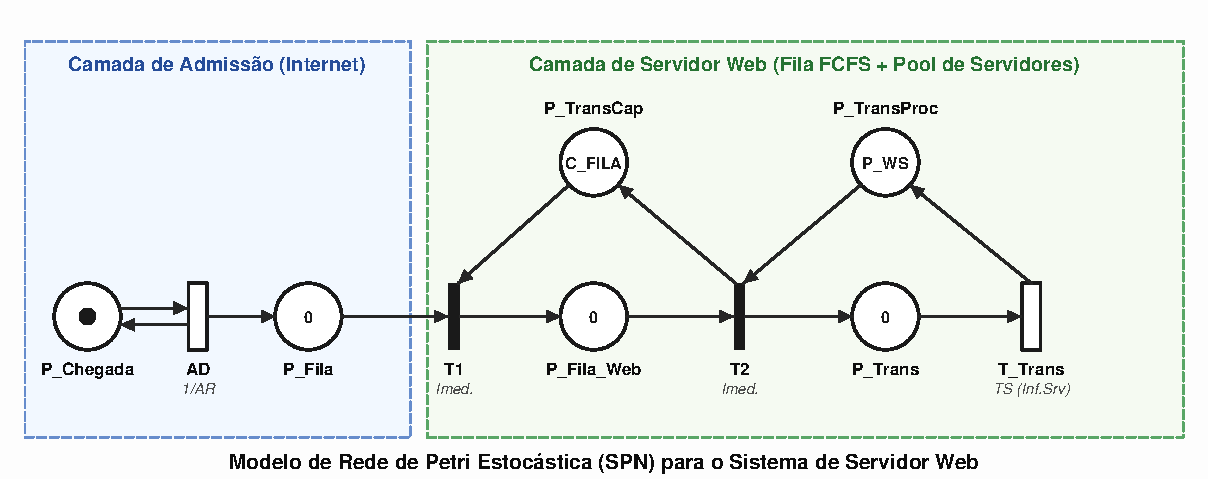
\includegraphics[width=\columnwidth]{fig_modelo_spn.pdf}
    \caption{Modelo SPN do sistema de Servidor Web com fila limitada ($C\_FILA$) e múltiplos núcleos de processamento ($P\_WS$).}
    \label{fig:spn}
\end{figure}

Na entrada do modelo, o lugar \texttt{P\_Chegada} começa com $1$ ficha e mantém a transição temporizada \texttt{AD} ativa. A transição \texttt{AD} dispara com tempo médio $AD = 1/AR$~ms (modo \textit{Single Server}), devolvendo uma ficha para \texttt{P\_Chegada} e colocando uma ficha em \texttt{P\_Fila}, que indica uma nova requisição pronta para entrar no sistema.

A entrada na fila do servidor depende do lugar \texttt{P\_TransCap}, que guarda o número de vagas livres no buffer e inicia com $C\_FILA$ fichas. Quando há vaga disponível ($\#\texttt{P\_TransCap} > 0$), a transição imediata \texttt{T1} dispara na hora, retira uma ficha de \texttt{P\_Fila} e uma de \texttt{P\_TransCap}, e coloca uma ficha em \texttt{P\_Fila\_Web}, representando a requisição esperando na fila. Se não houver ficha em \texttt{P\_TransCap} ($\#\texttt{P\_TransCap} = 0$), a fila está cheia e a requisição não entra, sendo contabilizada como descarte.

O atendimento pelos servidores é controlado pelo lugar \texttt{P\_TransProc}, que começa com $P\_WS$ fichas (total de núcleos livres). Quando existe requisição esperando em \texttt{P\_Fila\_Web} e pelo menos um núcleo livre em \texttt{P\_TransProc}, a transição imediata \texttt{T2} dispara. Esse disparo consome uma ficha de \texttt{P\_Fila\_Web} e uma de \texttt{P\_TransProc}, devolve uma ficha para \texttt{P\_TransCap} (liberando o espaço na fila de espera) e coloca uma ficha em \texttt{P\_Trans}, que indica a requisição sendo processada.

O tempo de execução no servidor é representado pela transição temporizada \texttt{T\_Trans}, configurada com tempo médio $TS = 20$~ms e semântica \textit{Infinite Server}. Com essa semântica, todas as requisições que estão em \texttt{P\_Trans} são processadas ao mesmo tempo por seus respectivos núcleos, com taxa total proporcional ao número de fichas ocupadas ($\#\texttt{P\_Trans} / TS$). Ao terminar o processamento, \texttt{T\_Trans} devolve a ficha para \texttt{P\_TransProc}, liberando o núcleo para a próxima requisição. A Tabela~\ref{tab:componentes} resume os elementos do modelo.

\begin{table}[htbp]
\centering
\caption{Lugares, Transições e Parâmetros do Modelo SPN}
\label{tab:componentes}
\renewcommand{\arraystretch}{1.12}
\setlength{\tabcolsep}{3.5pt}
\resizebox{\columnwidth}{!}{%
\begin{tabular}{llp{5.1cm}}
\toprule
\textbf{Tipo} & \textbf{Nome} & \textbf{Função no Modelo e Configuração} \\
\midrule
Lugar & \texttt{P\_Chegada} & Gera a chegada de requisições (Marcação inicial = $1$). \\
Lugar & \texttt{P\_Fila} & Requisição recém-chegada na entrada (Marcação inicial = $0$). \\
Lugar & \texttt{P\_TransCap} & Vagas livres na fila de espera (Marcação inicial = $C\_FILA$). \\
Lugar & \texttt{P\_Fila\_Web} & Requisições esperando na fila FCFS (Marcação inicial = $0$). \\
Lugar & \texttt{P\_TransProc} & Núcleos livres nos servidores Web (Marcação inicial = $P\_WS$). \\
Lugar & \texttt{P\_Trans} & Requisições em processamento ativo (Marcação inicial = $0$). \\
\midrule
Trans. & \texttt{AD} & Temporizada (\textit{Single Server}, Exponencial), atraso $AD = 1/AR$~ms. \\
Trans. & \texttt{T1} & Imediata (peso $1$). Aceita requisição na fila se $\#\texttt{P\_TransCap} > 0$. \\
Trans. & \texttt{T\_Descarte} & Imediata (peso $1$, guarda $\#\texttt{P\_TransCap} = 0$). Descarta se fila cheia. \\
Trans. & \texttt{T2} & Imediata (peso $1$). Aloca núcleo livre e libera vaga em \texttt{P\_TransCap}. \\
Trans. & \texttt{T\_Trans} & Temporizada (\textit{Infinite Server}, Exponencial), atraso $TS = 20$~ms. \\
\midrule
Parâm. & $AR$ / $AD$ & Taxa de chegada (req/ms) e tempo entre chegadas $AD = 1/AR$ (ms). \\
Parâm. & $P\_WS$ & Número total de núcleos dos servidores ($P\_WS \in \{4, 6, 8, 12, 16\}$). \\
Parâm. & $C\_FILA$ & Tamanho máximo da fila de espera ($C\_FILA \in \{10, 20, 40\}$). \\
Parâm. & $TS$ & Tempo médio de processamento em cada núcleo ($TS = 20$~ms). \\
\bottomrule
\end{tabular}%
}
\end{table}

\subsection{Métricas de Desempenho}
Foram definidas seis métricas para avaliar o modelo. Nas fórmulas abaixo, $\texttt{E}\{\#\texttt{Lugar}\}$ indica a média de fichas no lugar em regime estacionário e $\texttt{P}\{\text{condição}\}$ indica a probabilidade de a condição ocorrer:

\begin{enumerate}
    \item \textbf{Utilização ($U$, em \%)}: Percentual médio de núcleos ocupados processando requisições em relação ao total $P\_WS$:
    \begin{equation}
        U = \left(\frac{\texttt{E}\{\#\texttt{P\_Trans}\}}{P\_WS}\right) \times 100
        \label{eq:u}
    \end{equation}

    \item \textbf{Probabilidade de Descarte ($DP$, em \%)}: Percentual de requisições que chegam quando não há vagas na fila ($\#\texttt{P\_TransCap} = 0$) e são rejeitadas:
    \begin{equation}
        DP = \texttt{P}\{(\#\texttt{P\_Fila} > 0) \land (\#\texttt{P\_TransCap} = 0)\} \times 100
        \label{eq:dp}
    \end{equation}
    Como as chegadas seguem um processo de Poisson (propriedade PASTA), nas marcações tangíveis esse valor é igual a $\texttt{P}\{\#\texttt{P\_TransCap} = 0\} \times 100$.

    \item \textbf{Vazão (\textit{Throughput}, $TP$, em req/s)}: Quantidade média de requisições concluídas por segundo pela transição \texttt{T\_Trans}:
    \begin{equation}
        TP = \left(\frac{\texttt{E}\{\#\texttt{P\_Trans}\}}{TS}\right) \times 1000
        \label{eq:tp}
    \end{equation}

    \item \textbf{Tempo Médio de Resposta ($MRT$, em ms)}: Tempo médio total que uma requisição aceita gasta no sistema (fila mais processamento), obtido pela Lei de Little considerando a taxa efetiva de entrada $\lambda_{\text{ef}} = (1 - DP/100)/AD$:
    \begin{equation}
        MRT = \frac{\left(\texttt{E}\{\#\texttt{P\_Fila\_Web}\} + \texttt{E}\{\#\texttt{P\_Trans}\}\right) \times AD}{1 - \texttt{P}\{(\#\texttt{P\_Fila} > 0) \land (\#\texttt{P\_TransCap} = 0)\}}
        \label{eq:mrt}
    \end{equation}

    \item \textbf{Tempo Médio de Fila ($MQT$, em ms)}: Tempo médio que uma requisição aceita passa aguardando em \texttt{P\_Fila\_Web}:
    \begin{equation}
        MQT = \frac{\texttt{E}\{\#\texttt{P\_Fila\_Web}\} \times AD}{1 - \texttt{P}\{(\#\texttt{P\_Fila} > 0) \land (\#\texttt{P\_TransCap} = 0)\}}
        \label{eq:mqt}
    \end{equation}

    \item \textbf{Tempo Médio de Processamento ($MPT$, em ms)}: Tempo médio gasto apenas na etapa de execução em \texttt{P\_Trans}:
    \begin{equation}
        MPT = \frac{\texttt{E}\{\#\texttt{P\_Trans}\} \times AD}{1 - \texttt{P}\{(\#\texttt{P\_Fila} > 0) \land (\#\texttt{P\_TransCap} = 0)\}}
        \label{eq:mpt}
    \end{equation}
\end{enumerate}

A Tabela~\ref{tab:metricas} apresenta o resumo das seis métricas e suas expressões no Jupiter Analytics.

\begin{table}[htbp]
\centering
\caption{Expressões das Métricas Utilizados no Modelo SPN}
\label{tab:metricas}
\renewcommand{\arraystretch}{1.15}
\setlength{\tabcolsep}{3pt}
\resizebox{\columnwidth}{!}{%
\begin{tabular}{llp{5.8cm}}
\toprule
\textbf{Métrica} & \textbf{Unid.} & \textbf{Expressão no Modelo SPN} \\
\midrule
\texttt{U} & \% & \texttt{(E\{\#P\_Trans\}/P\_WS)*100} \\
\texttt{DP} & \% & \texttt{P\{(\#P\_Fila>0) and (\#P\_TransCap=0)\}*100} \\
\texttt{TP} & req/s & \texttt{(E\{\#P\_Trans\}/TS)*1000} \\
\texttt{MRT} & ms & \texttt{((E\{\#P\_Fila\_Web\}+E\{\#P\_Trans\})*AD)/(1-P\{\#P\_TransCap=0\})} \\
\texttt{MQT} & ms & \texttt{(E\{\#P\_Fila\_Web\}*AD)/(1-P\{\#P\_TransCap=0\})} \\
\texttt{MPT} & ms & \texttt{(E\{\#P\_Trans\}*AD)/(1-P\{\#P\_TransCap=0\})} \\
\bottomrule
\end{tabular}%
}
\end{table}

\section{Simulações e Resultados}

\subsection{Cenário de Referência e Planejamento dos Experimentos}
Os experimentos foram avaliados em \textbf{regime estacionário}, pois o modelo possui número finito de estados ($P\_WS + C\_FILA$) e atinge equilíbrio estatístico para todos os parâmetros testados. Os valores estacionários também foram conferidos por simulação de eventos discretos (\textit{Token Game}) no horizonte de $200.000$~ms.

O \textbf{Cenário de Referência} foi definido com os seguintes valores base:
\begin{itemize}
    \item \textbf{Tempo médio de serviço ($TS$)}: $20,0$~ms por requisição (cada núcleo processa em média $0,05$~req/ms ou $50$~req/s);
    \item \textbf{Capacidade de processamento ($P\_WS$)}: $8$~núcleos ($4$~máquinas com $2$~núcleos cada), resultando em capacidade máxima de $400$~req/s ($0,40$~req/ms);
    \item \textbf{Capacidade da fila ($C\_FILA$)}: $20$~posições na fila de espera;
    \item \textbf{Taxa de chegada padrão ($AR$)}: $0,40$~req/ms ($AD = 2,50$~ms, ou $400$~req/s), valor em que a taxa de chegada iguala a capacidade máxima dos 8 núcleos.
\end{itemize}

A partir do cenário de referência, foram realizados quatro conjuntos de experimentos:
\begin{itemize}
    \item \textbf{E1 (Taxa de chegada)}: $5$ níveis de demanda com $AR \in \{0,10;\ 0,25;\ 0,40;\ 0,55;\ 0,70\}$~req/ms (além da curva de $0,05$ a $0,80$~req/ms), mantendo $P\_WS = 8$ e $C\_FILA = 20$;
    \item \textbf{E2 (Capacidade de processamento)}: $3$ configurações de recursos com $P\_WS \in \{4\text{ (Config. A)},\ 8\text{ (Config. B)},\ 12\text{ (Config. C)}\}$~núcleos, mantendo $C\_FILA = 20$ e $AR = 0,40$~req/ms;
    \item \textbf{E3 (Capacidade da fila)}: $3$ limites de fila com $C\_FILA \in \{10,\ 20,\ 40\}$~vagas, mantendo $P\_WS = 8$ e $AR = 0,40$~req/ms;
    \item \textbf{E4 (Demanda e recursos combinados)}: $3$ cenários sob demanda alta ($AR = 0,55$~req/ms, ou $550$~req/s): \textbf{C1} com poucos recursos ($P\_WS = 6$, $C\_FILA = 10$), \textbf{C2} com recursos intermediários ($P\_WS = 12$, $C\_FILA = 20$) e \textbf{C3} com recursos elevados ($P\_WS = 16$, $C\_FILA = 40$).
\end{itemize}

A Tabela~\ref{tab:consolidada} reúne os parâmetros configurados e os resultados obtidos nos 14 testes realizados.

\begin{table*}[htbp]
\centering
\caption{Tabela Consolidada de Parâmetros e Resultados dos Experimentos E1, E2, E3 e E4 ($TS = 20,0$~ms)}
\label{tab:consolidada}
\renewcommand{\arraystretch}{1.12}
\setlength{\tabcolsep}{4pt}
\resizebox{\textwidth}{!}{%
\begin{tabular}{llccccccccccc}
\toprule
\textbf{Cód.} & \textbf{Cenário Experimental} & \textbf{$AR$ (req/ms)} & \textbf{$AD$ (ms)} & \textbf{$P\_WS$} & \textbf{$C\_FILA$} & \textbf{$\texttt{E}\{\#\texttt{P\_Fila\_Web}\}$} & \textbf{$\texttt{E}\{\#\texttt{P\_Trans}\}$} & \textbf{$U$ (\%)} & \textbf{$TP$ (req/s)} & \textbf{$MQT$ (ms)} & \textbf{$MPT$ (ms)} & \textbf{$MRT$ (ms)} & \textbf{$DP$ (\%)} \\
\midrule
E1.1 & Demanda Baixa ($100$~req/s) & 0,10 & 10,00 & 8 & 20 & 0,0003 & 2,0000 & 25,00 & 100,00 & 0,00 & 20,00 & 20,00 & 0,00 \\
E1.2 & Demanda Moderada ($250$~req/s) & 0,25 & 4,00 & 8 & 20 & 0,2779 & 5,0000 & 62,50 & 250,00 & 1,11 & 20,00 & 21,11 & 0,00 \\
E1.3 & Demanda Nominal / Ref. ($400$~req/s) & 0,40 & 2,50 & 8 & 20 & 8,6620 & 7,6701 & 95,88 & 383,50 & 22,59 & 20,00 & 42,59 & 4,12 \\
E1.4 & Demanda Alta ($550$~req/s) & 0,55 & 1,82 & 8 & 20 & 17,3447 & 7,9985 & 99,98 & 399,93 & 43,37 & 20,00 & 63,37 & 27,29 \\
E1.5 & Demanda Extrema ($700$~req/s) & 0,70 & 1,43 & 8 & 20 & 18,6665 & 8,0000 & 100,00 & 400,00 & 46,67 & 20,00 & 66,67 & 42,86 \\
\midrule
E2.1 & Config. A ($2$~Máq. $\times 2$~Núcleos) & 0,40 & 2,50 & 4 & 20 & 19,0000 & 4,0000 & 100,00 & 200,00 & 95,00 & 20,00 & 115,00 & 50,00 \\
E2.2 & Config. B ($4$~Máq. $\times 2$~Núcleos, Ref.) & 0,40 & 2,50 & 8 & 20 & 8,6620 & 7,6701 & 95,88 & 383,50 & 22,59 & 20,00 & 42,59 & 4,12 \\
E2.3 & Config. C ($6$~Máq. $\times 2$~Núcleos) & 0,40 & 2,50 & 12 & 20 & 0,2786 & 7,9997 & 66,67 & 399,99 & 0,70 & 20,00 & 20,70 & 0,00 \\
\midrule
E3.1 & Fila Curta ($C\_FILA = 10$) & 0,40 & 2,50 & 8 & 10 & 3,8606 & 7,4384 & 92,98 & 371,92 & 10,38 & 20,00 & 30,38 & 7,02 \\
E3.2 & Fila Média ($C\_FILA = 20$, Ref.) & 0,40 & 2,50 & 8 & 20 & 8,6620 & 7,6701 & 95,88 & 383,50 & 22,59 & 20,00 & 42,59 & 4,12 \\
E3.3 & Fila Longa ($C\_FILA = 40$) & 0,40 & 2,50 & 8 & 40 & 18,5329 & 7,8193 & 97,74 & 390,96 & 47,40 & 20,00 & 67,40 & 2,26 \\
\midrule
E4.1 & C1: Subdimensionado em Pico & 0,55 & 1,82 & 6 & 10 & 8,8055 & 5,9983 & 99,97 & 299,92 & 29,36 & 20,00 & 49,36 & 45,47 \\
E4.2 & C2: Equilibrado / Recomendado & 0,55 & 1,82 & 12 & 20 & 4,5729 & 10,8745 & 90,62 & 543,72 & 8,41 & 20,00 & 28,41 & 1,14 \\
E4.3 & C3: Superdimensionado & 0,55 & 1,82 & 16 & 40 & 0,2539 & 11,0000 & 68,75 & 550,00 & 0,46 & 20,00 & 20,46 & 0,00 \\
\bottomrule
\end{tabular}%
}
\end{table*}

\subsection{Resultados do Experimento E1 (Taxa de Chegada)}
A Figura~\ref{fig:e1} mostra o comportamento das métricas para taxas de chegada de $0,05$ a $0,80$~req/ms (com linhas tracejadas indicando os cinco pontos de E1.1 a E1.5). Nas Figuras~\ref{fig:e1}(a) e \ref{fig:e1}(b), quando a demanda é baixa ou moderada ($AR \le 0,25$~req/ms, em E1.1 e E1.2), a utilização $U$ e a vazão $TP$ crescem de forma linear. A utilização sobe de $25,00\%$ em E1.1 ($100$~req/s) para $62,50\%$ em E1.2 ($250$~req/s), sem ocorrer descarte ($DP = 0,00\%$).

\begin{figure}[htbp]
    \centering
    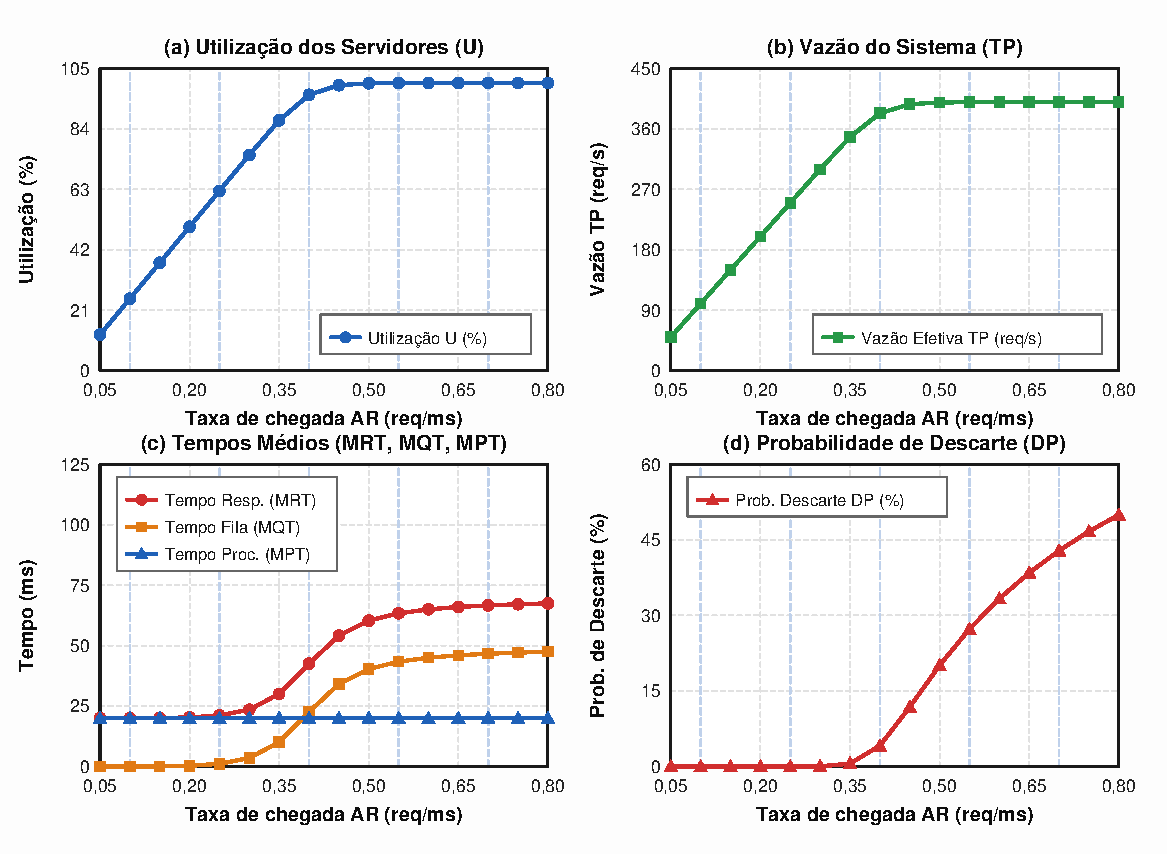
\includegraphics[width=\columnwidth]{fig_e1_demanda.pdf}
    \caption{Métricas do Experimento E1 variando a taxa de chegada $AR$ ($P\_WS = 8$, $C\_FILA = 20$): (a) Utilização $U$, (b) Vazão $TP$, (c) Tempos Médios $MRT$, $MQT$ e $MPT$, e (d) Probabilidade de Descarte $DP$.}
    \label{fig:e1}
\end{figure}

Quando a chegada alcança $AR = 0,40$~req/ms (E1.3), a utilização dos 8 núcleos chega a $95,88\%$ e a fila passa a acumular em média $8,66$ requisições. Na Figura~\ref{fig:e1}(c), o tempo médio de processamento ($MPT$) continua fixo em $20,00$~ms em todos os testes, porque cada requisição que entra em \texttt{P\_Trans} é atendida por um núcleo dedicado. Já o tempo médio de fila ($MQT$) sobe de $1,11$~ms (E1.2) para $22,59$~ms (E1.3) e chega a $46,67$~ms em E1.5 ($AR = 0,70$~req/ms), elevando o $MRT$ de $20,00$~ms para $66,67$~ms. Na Figura~\ref{fig:e1}(d), como a vazão máxima dos 8 núcleos trava em $400,00$~req/s a partir de $AR = 0,50$~req/ms, as requisições excedentes encontram a fila cheia e o descarte sobe para $27,29\%$ em E1.4 e $42,86\%$ em E1.5.

\subsection{Resultados do Experimento E2 (Capacidade de Processamento)}
A Figura~\ref{fig:e2} apresenta os resultados ao variar o número de núcleos $P\_WS \in \{4, 8, 12\}$. Na Configuração A ($P\_WS = 4$, teste E2.1), os 4 núcleos conseguem atender no máximo $200$~req/s ($0,20$~req/ms). Como a taxa de chegada padrão é o dobro disso ($AR = 0,40$~req/ms), o sistema satura completamente: a utilização fica em $100,00\%$, metade das requisições é perdida ($DP = 50,00\%$), a fila mantém média de $19,00$ requisições ocupadas e o tempo de resposta chega a $115,00$~ms ($MQT = 95,00$~ms).

\begin{figure}[htbp]
    \centering
    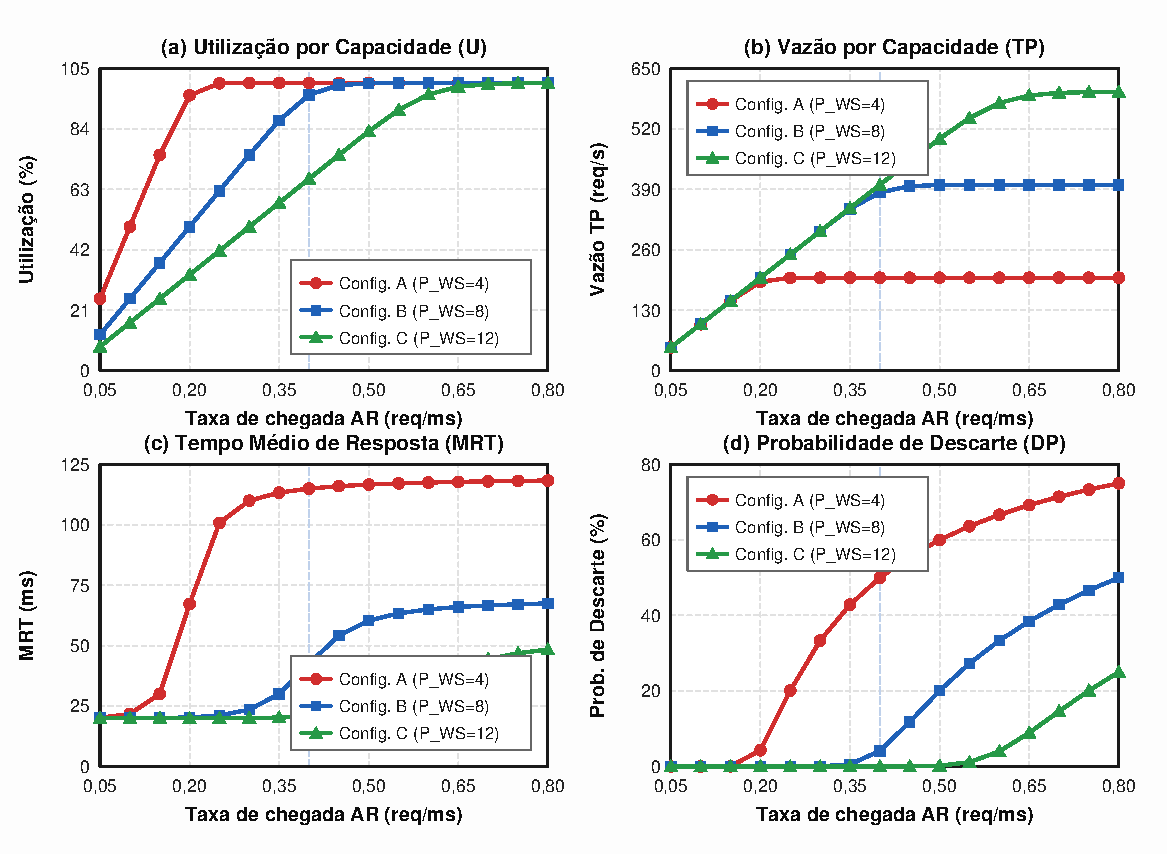
\includegraphics[width=\columnwidth]{fig_e2_capacidade.pdf}
    \caption{Métricas do Experimento E2 variando a capacidade de processamento ($P\_WS \in \{4, 8, 12\}$, com $C\_FILA = 20$): (a) Utilização $U$, (b) Vazão $TP$, (c) Tempo Médio de Resposta $MRT$ e (d) Descarte $DP$.}
    \label{fig:e2}
\end{figure}

Com $P\_WS = 8$ núcleos na Configuração B (E2.2), a vazão sobe para $383,50$~req/s, o $MRT$ cai para $42,59$~ms e o descarte diminui para $4,12\%$. Ao passar para $P\_WS = 12$ núcleos na Configuração C (E2.3), a capacidade máxima do sistema sobe para $600$~req/s. Para a taxa de chegada de $400$~req/s, a utilização fica em $66,67\%$, não há perda de pacotes ($DP = 0,00\%$), a vazão alcança $399,99$~req/s e o tempo de espera na fila cai para $0,70$~ms ($MRT = 20,70$~ms).

\subsection{Resultados do Experimento E3 (Capacidade da Fila)}
A Figura~\ref{fig:e3} mostra o efeito de alterar o tamanho máximo da fila $C\_FILA \in \{10, 20, 40\}$ mantendo fixos $P\_WS = 8$ núcleos. Em $AR = 0,40$~req/ms, aumentar a fila de $10$ (E3.1) para $40$ posições (E3.3) reduz o descarte de $7,02\%$ para $2,26\%$, mas faz o tempo médio de resposta subir $121,8\%$ (de $30,38$~ms para $67,40$~ms, passando de $118$~ms quando $AR \ge 0,60$~req/ms). Além disso, na Figura~\ref{fig:e3}(b), para taxas acima de $0,50$~req/ms as três curvas de descarte ficam sobrepostas, mostrando que aumentar apenas a fila sem aumentar os núcleos de processamento só deixa as requisições esperando mais tempo antes de o buffer lotar novamente.

\begin{figure}[htbp]
    \centering
    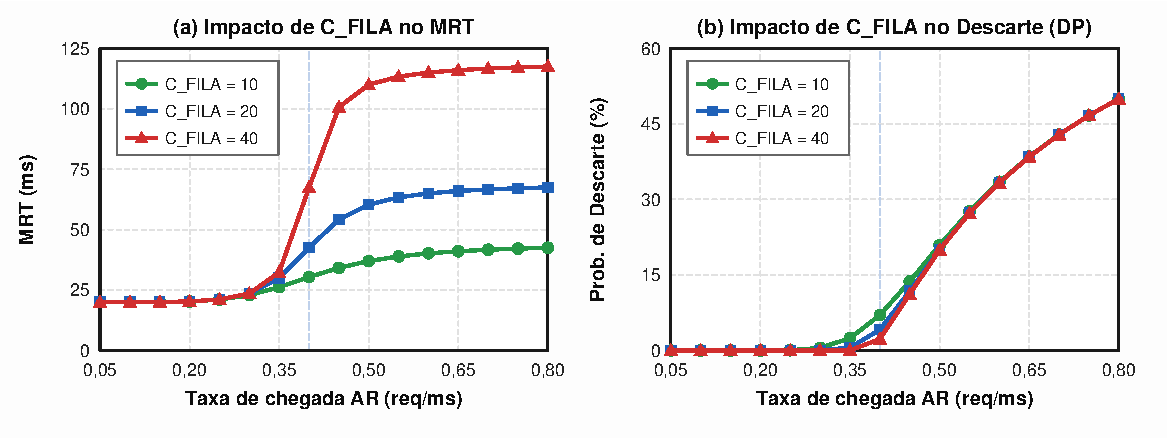
\includegraphics[width=\columnwidth]{fig_e3_fila.pdf}
    \caption{Métricas do Experimento E3 variando o limite da fila $C\_FILA \in \{10, 20, 40\}$ ($P\_WS = 8$): (a) $MRT$ e (b) Probabilidade de Descarte $DP$.}
    \label{fig:e3}
\end{figure}

\subsection{Resultados do Experimento E4 e Discussão das Questões}
A Figura~\ref{fig:e4} compara os três cenários combinados (C1, C2 e C3) submetidos a uma demanda alta de $AR = 0,55$~req/ms ($550$~req/s). A partir dos dados obtidos nos quatro experimentos, é possível responder às cinco questões propostas para a avaliação do sistema:

\begin{figure}[htbp]
    \centering
    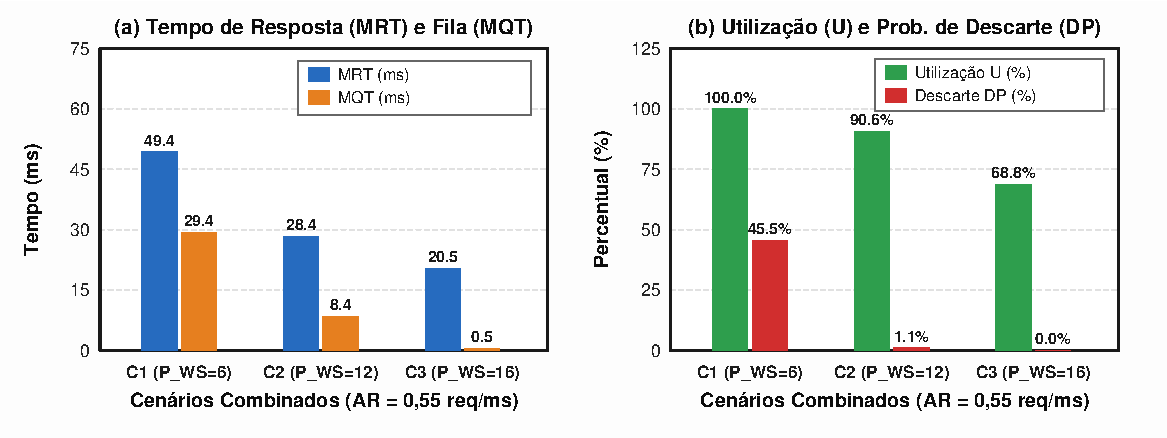
\includegraphics[width=\columnwidth]{fig_e4_combinado.pdf}
    \caption{Comparação dos cenários C1, C2 e C3 do Experimento E4 sob demanda de $AR = 0,55$~req/ms: (a) $MRT$ e $MQT$, e (b) Utilização $U$ e Descarte $DP$.}
    \label{fig:e4}
\end{figure}

\textbf{(i) Como a demanda influencia o desempenho?} Enquanto a taxa de chegada $AR$ está abaixo da capacidade máxima dos servidores ($P\_WS / TS$), o aumento da demanda faz a utilização e a vazão crescerem na mesma proporção, mantendo o tempo de resposta próximo ao tempo de serviço ($20$~ms) e o descarte em zero. Quando a demanda alcança ou passa desse limite, os núcleos chegam a $100\%$ de uso, a vazão para de crescer, a fila enche rapidamente e tanto o tempo de espera ($MQT$) quanto a taxa de descarte ($DP$) sobem de forma acentuada.

\textbf{(ii) Qual o principal gargalo?} O principal gargalo está na \textbf{quantidade de núcleos de processamento dos servidores Web} (lugar \texttt{P\_TransProc}, definido por $P\_WS$). Quando todas as fichas de \texttt{P\_TransProc} estão ocupadas em \texttt{P\_Trans}, a transição \texttt{T2} não consegue retirar novas requisições de \texttt{P\_Fila\_Web}, o que faz a fila encher até esgotar as fichas de \texttt{P\_TransCap} e provocar descartes.

\textbf{(iii) Qual o efeito do aumento da capacidade?} Aumentar a capacidade de processamento ($P\_WS$ em E2) aumenta diretamente a vazão máxima suportada e reduz o tempo de fila e o descarte. Já aumentar apenas a capacidade da fila ($C\_FILA$ em E3) ajuda a reduzir pequenas perdas quando a carga está próxima do limite dos servidores, mas aumenta bastante o tempo de resposta ($MRT$) quando o tráfego continua alto.

\textbf{(iv) Qual configuração equilibra recursos e desempenho?} Na Figura~\ref{fig:e4}, o cenário \textbf{C1} ($P\_WS = 6$, $C\_FILA = 10$) não suporta a demanda de $550$~req/s e descarta $45,47\%$ das requisições, com $MRT$ de $49,36$~ms. O cenário \textbf{C3} ($P\_WS = 16$, $C\_FILA = 40$) zera o descarte e baixa o $MRT$ para $20,46$~ms, mas opera com $31,25\%$ dos núcleos ociosos ($U = 68,75\%$) usando 4 núcleos e 20 posições de fila a mais que o C2. O cenário \textbf{C2} ($P\_WS = 12$, $C\_FILA = 20$) mantém boa ocupação dos servidores ($U = 90,62\%$), atende $543,72$~req/s ($98,86\%$ da demanda), entrega $MRT$ baixo ($28,41$~ms) e tem descarte de apenas $1,14\%$.

\textbf{(v) Qual configuração é recomendada e por quê?} A configuração recomendada é a de \textbf{$P\_WS = 12$ núcleos (6 máquinas com 2 núcleos) e fila $C\_FILA = 20$}, avaliada em \textbf{E2.3} e \textbf{E4.2 (C2)}. Ela é a mais indicada porque atende a carga nominal de $400$~req/s sem nenhum descarte e com $MRT$ de $20,70$~ms, além de suportar picos de $550$~req/s reduzindo o tempo de resposta em $42,4\%$ em relação a C1, sem o gasto extra de manter 16 núcleos como em C3 (que aumentaria a vazão em apenas $1,15\%$).

\section{Conclusão}
Este trabalho apresentou um modelo de Rede de Petri Estocástica (SPN) construído no Jupiter Analytics para avaliar o desempenho de um sistema de Servidor Web com fila limitada. Foram avaliadas seis métricas ($TP$, $MRT$, $MQT$, $MPT$, $U$ e $DP$) em quatro baterias de experimentos (E1 a E4) variando a demanda, o número de núcleos e o limite da fila.

Os experimentos mostraram que a limitação de núcleos de processamento (\texttt{P\_TransProc}) é o gargalo central da arquitetura. Configurações com poucos núcleos ($P\_WS = 4$ ou $6$) chegaram a descartar entre $45,47\%$ e $50,00\%$ das requisições, enquanto o aumento isolado da fila para $40$ posições dobrou o tempo médio de resposta sem aumentar a vazão máxima. A configuração com $P\_WS = 12$ núcleos e $C\_FILA = 20$ posições teve o melhor equilíbrio entre desempenho e quantidade de recursos, mantendo $MRT$ de $20,70$~ms sem perdas na carga nominal e $MRT$ de $28,41$~ms com $1,14\%$ de perda sob tráfego de pico.

Como trabalhos futuros, o modelo pode ser expandido para incluir uma camada de banco de dados e servidores de cache, além de avaliar falhas e recuperação de máquinas do cluster.

\section*{Repositório GitHub e Vídeo de Apresentação}
Os arquivos de configuração do modelo SPN, o notebook utilizado nos experimentos, as tabelas CSV de resultados e o vídeo de apresentação de 5 minutos estão disponíveis nos links a seguir:
\begin{itemize}
    \item \textbf{GitHub}: \url{https://github.com/outbreakufpi/Trabalho07SD}
    \item \textbf{Vídeo (5 min)}: \url{https://youtu.be/LINK_DO_VIDEO}
\end{itemize}

\begin{thebibliography}{00}
\bibitem{menasce2002} D. A. Menascé and V. A. F. Almeida, \textit{Capacity Planning for Web Services: Metrics, Models, and Methods}, 1st ed. Upper Saddle River, NJ, USA: Prentice Hall PTR, 2002.
\bibitem{cao2003} J. Cao, M. Andersson, C. Nyberg, and M. Kihl, ``Web server performance modeling using an M/G/1/K*PS queue,'' in \textit{Proc. 10th International Conference on Telecommunications (ICT)}, Papeete, Tahiti, 2003, vol. 2, pp. 1501-1506.
\bibitem{santos2021} L. Santos, B. Cunha, I. Fé, M. Vieira, and F. A. Silva, ``Data processing on edge and cloud: a performability evaluation and sensitivity analysis,'' \textit{Journal of Network and Systems Management}, vol. 29, no. 3, pp. 1-24, 2021.
\bibitem{macedo2022} J. Macêdo, V. Carvalho, E. Andrade, and F. A. Silva, ``Modelagem e Análise da Comunicação em VANETs com uso de RSUs,'' in \textit{Anais do XXI Workshop em Desempenho de Sistemas Computacionais e de Comunicação (WPerformance)}, Sociedade Brasileira de Computação (SBC), 2022, pp. 1-12.
\bibitem{bolch2006} G. Bolch, S. Greiner, H. de Meer, and K. S. Trivedi, \textit{Queueing Networks and Markov Chains: Modeling and Performance Evaluation with Computer Science Applications}, 2nd ed. Hoboken, NJ, USA: John Wiley \& Sons, 2006.
\bibitem{marsan1995} M. A. Marsan, G. Balbo, G. Conte, S. Donatelli, and G. Franceschinis, \textit{Modelling with Generalized Stochastic Petri Nets}, 1st ed. Chichester, UK: John Wiley \& Sons, 1995.
\bibitem{oliveira2017} D. Oliveira, R. Matos, J. Dantas, J. Ferreira, B. Silva, G. Callou, P. Maciel, and A. Brinkmann, ``Advanced stochastic petri net modeling with the mercury scripting language,'' in \textit{Proc. 11th EAI International Conference on Performance Evaluation Methodologies and Tools (VALUETOOLS)}, Venice, Italy, 2017, pp. 192-197.
\bibitem{jupiter2024} PASID, ``Jupiter Analytics: Ambiente de Modelagem e Simulação de Redes de Petri Estocásticas,'' Universidade Federal do Piauí (UFPI), 2024. [Online]. Available: \url{https://jupiteranalytics.com.br}
\end{thebibliography}

\end{document}
